\documentclass[tikz,border=5mm]{standalone}
\usepackage{fontspec}
\setmainfont{Hiragino Sans}
\usepackage{xcolor}

\begin{document}
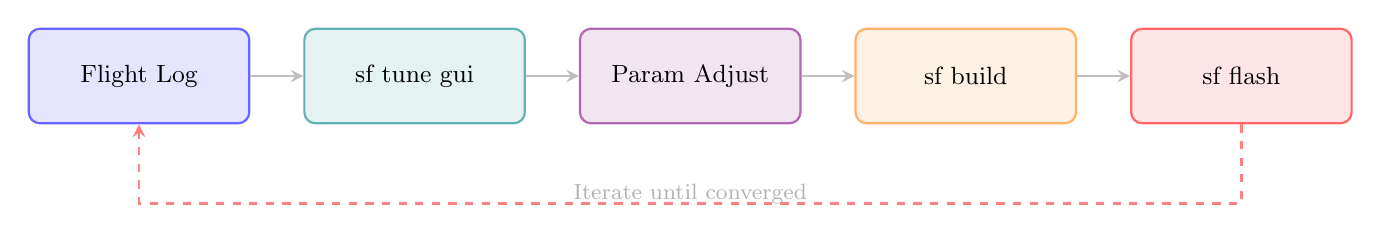
\begin{tikzpicture}[
  step/.style={
    draw=#1!60, fill=#1!10, rounded corners=4pt,
    minimum width=28mm, minimum height=12mm,
    font=\small, align=center, line width=0.8pt
  },
  arr/.style={
    ->, thick, color=gray!50, >=stealth, line width=1pt
  },
  cyc/.style={
    ->, thick, color=red!50, >=stealth, line width=1pt, dashed
  }
]

% Steps in a cycle
\node[step=blue]   (log)   at (0, 0)   {Flight Log};
\node[step=teal]   (tune)  at (3.5, 0) {sf tune gui};
\node[step=violet] (adj)   at (7, 0)   {Param Adjust};
\node[step=orange] (build) at (10.5, 0){sf build};
\node[step=red]    (flash) at (14, 0)  {sf flash};

% Forward arrows
\draw[arr] (log.east)   -- (tune.west);
\draw[arr] (tune.east)  -- (adj.west);
\draw[arr] (adj.east)   -- (build.west);
\draw[arr] (build.east) -- (flash.west);

% Feedback loop
\draw[cyc] (flash.south) -- ++(0, -1) -| (log.south);

% Labels
\node[font=\footnotesize, text=gray!60] at (7, -1.5) {Iterate until converged};

\end{tikzpicture}
\end{document}
